\documentclass[11pt,aspectratio=169]{beamer}

\usepackage[T1]{fontenc}
\usepackage{lmodern}
\usepackage{graphicx}
\usepackage{tikz}
\usetikzlibrary{arrows.meta,positioning,calc,decorations.pathreplacing,overlay-beamer-styles,shapes.geometric,patterns}
\usepackage{pgfplots}
\pgfplotsset{compat=1.17}
\usepackage{amsmath,amssymb,mathtools}
\usepackage{booktabs,tabularx,array,multirow}
\usepackage{appendixnumberbeamer}

\setbeamercovered{transparent=5}
\setbeamertemplate{navigation symbols}{}
\setbeamertemplate{itemize items}[circle]
\setbeamertemplate{itemize subitem}{--}
\setbeamertemplate{footline}[frame number]
\setbeamerfont{framesubtitle}{size=\small}
\setbeamercolor{block title}{fg=black,bg=white!80!black}
\setbeamercolor{block body}{fg=black,bg=white!97!black}
\linespread{1.2}

\newcolumntype{Y}{>{\raggedright\arraybackslash}X}
\newcolumntype{C}{>{\centering\arraybackslash}X}
\newcommand{\1}{\mathbf 1}
\newcommand{\E}{\mathbb E}
\newcommand{\sym}[1]{\ifmmode^{#1}\else\(^{#1}\)\fi}
\definecolor{citecolor}{RGB}{110,110,165}
\definecolor{sourcegray}{RGB}{95,95,95}
\newcommand{\cit}[1]{{\color{citecolor}#1}}
\newcommand{\source}[1]{\par\vspace{0.25em}{\tiny\color{sourcegray}Source: #1}}
\newcommand{\takeaway}[1]{\vfill{\small\textbf{Takeaway.} #1}}
\newcommand{\baselinefigure}{../output/model/e5f_pf_person_policy_rebated-tax1-baseline_20260826a_h128_convergence/diagnostics.pdf}

\title{Fertility and Housing Tenure Choice}
\author{Tommaso De Santo}
\date{September 14, 2026}

\begin{document}

{
\setbeamertemplate{footline}{}
\maketitle
}

\begin{frame}{Housing and Fertility}
\begin{center}
\includegraphics[width=0.45\textwidth]{../../Latex/newsweek.png}\hspace{-1em}%
\includegraphics[width=0.45\textwidth]{../../Latex/housingwire.png}\\[-0.8em]
\includegraphics[width=0.45\textwidth]{../../Latex/vox.png}\hspace{-1em}%
\includegraphics[width=0.45\textwidth]{../../Latex/cityjournal.png}
\includegraphics[width=0.8\textwidth]{../../Latex/times.png}
\end{center}
\end{frame}

\begin{frame}{Housing, Fertility, and Tenure Choice}
\textbf{Children increase how much physical space a household needs.}
Access to that space depends on tenure and wealth:
\begin{itemize}\setlength\itemsep{0.6em}
  \item Rental housing can limit the size of the home a family can occupy.
  \item Ownership expands the housing menu but requires liquid wealth for a down payment.
  \item Older owners may retain family-sized homes after their children leave.
\end{itemize}

\vfill
How much does access to family-sized housing affect fertility?\\
Which housing constraints matter, and for whom?
\end{frame}

\begin{frame}{This Paper}
Need a framework where fertility, tenure, housing size, saving, and population are jointly determined.

\vfill
\alert{First:} a simplified model of family space and tenure
\begin{itemize}
  \item Show when reallocating housing toward the young improves welfare at fixed fertility.
  \item Give a household condition for better housing access to raise fertility.
\end{itemize}

\vfill
\alert{Then:} a quantitative lifecycle model
\begin{itemize}
  \item Add sequential fertility, income risk, saving, housing adjustment, and bequests.
  \item Distinguish births, resident persons, household heads, and housing demand.
\end{itemize}

\vfill
\alert{Finally:} discipline the model and use it to study demographic and housing-market dynamics.
\end{frame}

\section{Simple Theory}

\begin{frame}[plain,c,noframenumbering]
\centering
{\Large\textbf{Simple Theory}}
\end{frame}

% Seven main theory frames; the September 14 deck is the presentation source.
\begin{frame}{Environment and Preferences}
\relax
\small\linespread{1.05}\selectfont
\setlength{\abovedisplayskip}{4pt}
\setlength{\belowdisplayskip}{4pt}
\setlength{\abovedisplayshortskip}{4pt}
\setlength{\belowdisplayshortskip}{4pt}
A two-period OLG economy: $Y_t$ young and $O_t$ old share a fixed housing stock $\bar H$.
\begin{itemize}\setlength\itemsep{0.3em}
  \item Entrants have young income $y_i^y$, liquid wealth $b_i$, and known old income $y_i^o$.
  \item Young choose consumption, housing, fertility, saving, and tenure; old may resize.
  \item Rentals satisfy $h\le h_R^{\max}$; owners satisfy $h\le h_O^{\max}$, with $h_R^{\max}<h_O^{\max}$.
\end{itemize}
\smallskip
Households value consumption, housing, children, and an estate:
\[
\begin{aligned}
u_t^y(c,h,n)&=\log(c-\chi n)+\alpha\log(h-\kappa n)+\vartheta_t\log n,\\[0.2em]
u^o(c^o,h^o,e)&=\log c^o+\gamma\log h^o+\omega_B\log e.
\end{aligned}
\]
{\small Each child requires $\chi$ goods and $\kappa$ space. Households discount future utility by $\beta$; $n>0$ is continuous.\par}
\vfill
{\small $(y_i^y,b_i,y_i^o)\sim F$. An independent logistic taste $\xi_i$ favors ownership; tenure is retained when old.\par}
\end{frame}

\begin{frame}[label=theory-households]{Household Choices}
\relax
\small\linespread{1.05}\selectfont
\setlength{\abovedisplayskip}{4pt}
\setlength{\belowdisplayskip}{4pt}
\setlength{\abovedisplayshortskip}{4pt}
\setlength{\belowdisplayshortskip}{4pt}
{\small Bonds cost $q\in(0,1)$, houses cost $P_t$, and rent $r_t$ is paid at period end. Property tax $\tau_t^p$ funds an equal rebate $T_t$.\par}
\smallskip
{\small Young maximize $u_t^y+\beta V_{t+1}^d$ over $(c,h,n,a')$, subject to:}
{\small
\small\linespread{1.05}\selectfont
\setlength{\abovedisplayskip}{4pt}
\setlength{\belowdisplayskip}{4pt}
\setlength{\abovedisplayshortskip}{4pt}
\setlength{\belowdisplayshortskip}{4pt}
\[
\begin{array}{rll}
\text{Rent:}&c+qa'+qr_t h=y_i^y+b_i+T_t,&a'\ge0,\\[0.35em]
\text{Own:}&c+qa'+(1+q\tau_t^p)P_t h=y_i^y+b_i+T_t,
&qa'+\phi_tP_t h\ge0.
\end{array}
\]
}
{\small Here $a'$ is next-period net financial wealth. A mortgage finances at most the share $\phi_t$ of the purchase price; current income and wealth fund the down payment.\par}
\medskip
{\small Old maximize $u^o$ over $(c^o,h^o,e)$; $H$ denotes inherited housing:}
{\small
\small\linespread{1.05}\selectfont
\setlength{\abovedisplayskip}{4pt}
\setlength{\belowdisplayskip}{4pt}
\setlength{\abovedisplayshortskip}{4pt}
\setlength{\belowdisplayshortskip}{4pt}
\[
c^o+qe+qr_t h^o=a+P_tH+y_i^o+T_t,
\qquad e\ge P_{t+1}h^o\ \text{for owners}.
\]
}
{\small Renters have $H=0$. The estate is $e=a^e/q+P_{t+1}h^o$ for owners and $e=a^e/q$ for renters, with financial saving $a^e\ge0$.\par}
\vfill
{\small Both ages respect their tenure's size limit. Young own if $W_t^O(i)+\xi_i\ge W_t^R(i)$.\hfill\hyperlink{theory-young-problems}{\beamerbutton{Problems}}\par}
\end{frame}

\begin{frame}{Competitive Equilibrium}
\relax
\small\linespread{1.05}\selectfont
\setlength{\abovedisplayskip}{4pt}
\setlength{\belowdisplayskip}{4pt}
\setlength{\abovedisplayshortskip}{4pt}
\setlength{\belowdisplayshortskip}{4pt}
{\small Given policies and initial cohorts and assets, prices, rebates and household choices satisfy optimality, rental competition, and market clearing:}
\[
\begin{aligned}
qr_t&=(1+q\tau_t^p)P_t-qP_{t+1}>0,\\[0.3em]
Y_t\bar h_t^y+O_t\bar h_t^o&=\bar H,\\[0.3em]
(Y_t+O_t)T_t&=q\tau_t^pP_t\bar H.
\end{aligned}
\]
{\small Bars denote averages over endowments and chosen tenure. Young choices determine next period's old assets and housing.\par}
\medskip
Each child generates $\nu$ entering households; cohort sizes follow:
\[
Y_{t+1}=\nu\bar n_tY_t,\qquad O_{t+1}=Y_t.
\]
\vfill
{\small A positive steady state has constant prices, choices and distributions, with $Y=O=N$, $\bar n=1/\nu$, and $N=\bar H/(\bar h^y+\bar h^o)$.\par}
\end{frame}

\begin{frame}[label=theory-allocation]{The Planner's Allocation}
\relax
\small\linespread{1.05}\selectfont
\setlength{\abovedisplayskip}{4pt}
\setlength{\belowdisplayskip}{4pt}
\setlength{\abovedisplayshortskip}{4pt}
\setlength{\belowdisplayshortskip}{4pt}
{\small At a stationary equilibrium, fix fertility, tenure, future opportunities, and net estates. Give each living household equal weight and choose all current consumption and housing:}
{\small
\small\linespread{1.05}\selectfont
\setlength{\abovedisplayskip}{4pt}
\setlength{\belowdisplayskip}{4pt}
\setlength{\abovedisplayshortskip}{4pt}
\setlength{\belowdisplayshortskip}{4pt}
\[
\begin{aligned}
\max_{\{c_i^y,h_i^y,c_i^o,h_i^o\}}\quad
&\int\!\left[u^y(c_i^y,h_i^y,n_i)+u^o(c_i^o,h_i^o,e_i)\right]\,\mathrm dQ\\
\text{s.t.}\quad
&\int(c_i^y+c_i^o)\,\mathrm dQ=C^{eq}/N,\quad
\int(h_i^y+h_i^o)\,\mathrm dQ=\bar H/N,\\
&h_i^y,h_i^o\le h_{d_i}^{\max}.
\end{aligned}
\]
}
{\footnotesize $Q$ is the common distribution of endowments and retained tenure; each age has mass $N$. $C^{eq}$ is total consumption in the reference equilibrium. Individual financial constraints may be relaxed.\par}
\medskip
{\small\textbf{Housing allocation.} If the planner's size limits are slack:}
\[
\bar h^{y,F}>\bar h^{y,eq}
\quad\Longleftrightarrow\quad
\alpha\bar h^{o,eq}>\gamma\bigl(\bar h^{y,eq}-\kappa\bar n\bigr).
\]
{\small The planner gives more housing to the young when their space after children's needs is low relative to old housing.\par}
\vfill
{\footnotesize\hyperlink{theory-planner-solution}{\beamerbutton{Allocation and caps}}\quad\hyperlink{theory-primitives}{\beamerbutton{An income condition}}\par}
\end{frame}

\begin{frame}{Housing Allocation}
\relax
\small\linespread{1.05}\selectfont
\setlength{\abovedisplayskip}{4pt}
\setlength{\belowdisplayskip}{4pt}
\setlength{\abovedisplayshortskip}{4pt}
\setlength{\belowdisplayshortskip}{4pt}
\begin{center}
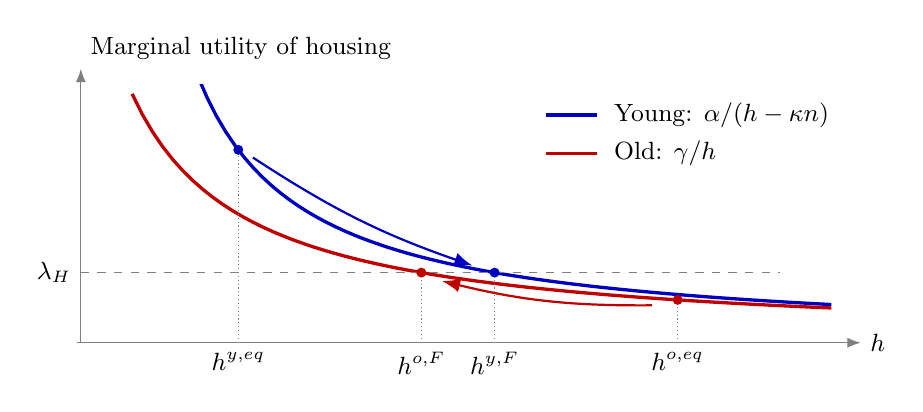
\begin{tikzpicture}[x=.93cm,y=4.9cm,>=Latex,font=\small]
\draw[->,gray] (.8,0)--(11.5,0) node[right,black] {$h$};
\draw[->,gray] (.85,0)--(.85,.71) node[above right,black] {Marginal utility of housing};
\begin{scope}\clip (.86,.005) rectangle (11.2,.67);
\draw[blue!75!black,very thick,domain=2.45:11.1,samples=70] plot(\x,{1/(\x-1)});
\draw[red!75!black,very thick,domain=1.55:11.1,samples=70] plot(\x,{1/\x});
\end{scope}
\draw[gray,dashed] (.85,{2/11})--(10.4,{2/11});
\node[left] at (.85,{2/11}) {$\lambda_H$};
\draw[gray,densely dotted] (3,0)--(3,.5);
\draw[gray,densely dotted] (5.5,0)--(5.5,{2/11});
\draw[gray,densely dotted] (6.5,0)--(6.5,{2/11});
\draw[gray,densely dotted] (9,0)--(9,{1/9});
\fill[blue!75!black] (3,.5) circle(1.8pt) (6.5,{2/11}) circle(1.8pt);
\fill[red!75!black] (9,{1/9}) circle(1.8pt) (5.5,{2/11}) circle(1.8pt);
\draw[->,blue!75!black,thick] (3.2,.48) to[bend right=7] (6.2,.20);
\draw[->,red!75!black,thick] (8.65,.097) to[bend left=7] (5.78,.16);
\node[below] at (3,0) {$h^{y,eq}$};
\node[below] at (5.5,0) {$h^{o,F}$};
\node[below] at (6.5,0) {$h^{y,F}$};
\node[below] at (9,0) {$h^{o,eq}$};
\draw[blue!75!black,very thick] (7.2,.59)--(7.9,.59);
\node[right] at (8,.59) {Young: $\alpha/(h-\kappa n)$};
\draw[red!75!black,very thick] (7.2,.49)--(7.9,.49);
\node[right] at (8,.49) {Old: $\gamma/h$};
\end{tikzpicture}
\end{center}
{\small The curves illustrate one young household and one old household, with $n=1$. For $\alpha=\gamma$ and slack planner limits:}
\[
\bar h^{y,F}-\bar h^{y,eq}
=\tfrac12\!\left[\kappa\bar n-\bigl(\bar h^{y,eq}-\bar h^{o,eq}\bigr)\right].
\]
{\small Young families gain space if their larger needs exceed their additional housing in equilibrium.\par}
\end{frame}

\begin{frame}[label=theory-fertility]{Housing and Fertility}
\relax
\small\linespread{1.05}\selectfont
\setlength{\abovedisplayskip}{4pt}
\setlength{\belowdisplayskip}{4pt}
\setlength{\abovedisplayshortskip}{4pt}
\setlength{\belowdisplayshortskip}{4pt}
Given its consumption and home, a parent chooses fertility to satisfy:
\[
\frac{\vartheta}{n}
=\underbrace{\frac{\chi}{c-\chi n}}_{\text{cost in goods}}
+\underbrace{\frac{\alpha\kappa}{h-\kappa n}}_{\text{cost in space}}.
\]
A larger home lowers the space cost of another child; more consumption lowers its goods cost.
\medskip
For a small change in the household's bundle, fertility rises exactly when:
\[
\frac{\chi}{(c-\chi n)^2}\,\mathrm dc
+\frac{\alpha\kappa}{(h-\kappa n)^2}\,\mathrm dh>0.
\]
The housing gain must outweigh any accompanying loss of consumption.
\vfill
{\small A policy must determine both changes.\hfill\hyperlink{theory-fertility-proof}{\beamerbutton{Derivation}}\quad\hyperlink{theory-joint-fertility}{\beamerbutton{Joint planner}}\par}
\end{frame}

\begin{frame}[label=theory-transition]{Demographic Transition}
\relax
\small\linespread{1.05}\selectfont
\setlength{\abovedisplayskip}{4pt}
\setlength{\belowdisplayskip}{4pt}
\setlength{\abovedisplayshortskip}{4pt}
\setlength{\belowdisplayshortskip}{4pt}
{\small A small permanent decline in the desire for children starts the baseline transition. At $I$, a small unexpected rebated property-tax increase starts from the same inherited state.\par}
\smallskip
{\centering

\includegraphics[width=\textwidth,height=0.53\textheight,keepaspectratio]{../output/model/simplified_olg_amendments/consolidated_transition_figure.pdf}\par}
\smallskip
{\small Under the local equilibrium conditions, the reform raises fertility on impact and leads to more adult households at the terminal steady state. Both steady states have $\bar n=1/\nu$.\par}
\vfill
{\footnotesize $S_-$ is the initial steady state; $S_0$ the baseline endpoint; $S_1$ the policy endpoint.\hfill\hyperlink{theory-transition-conditions}{\beamerbutton{Conditions}}\quad\hyperlink{theory-transition-curves}{\beamerbutton{Population}}\par}
\end{frame}

\section{Quantitative Model}

\begin{frame}[plain,c,noframenumbering]
\centering
{\Large\textbf{Quantitative Model}}
\end{frame}

\begin{frame}{Environment}
\begin{itemize}\setlength\itemsep{0.35em}
  \item Households live for a finite number of periods in one housing market.
  \item Beginning-of-period state:
  \[
    x=(b,z,a,h,n,m)
  \]
  \begin{itemize}
    \item $b$: liquid net wealth; $z$: earnings state; $a$: age
    \item $h$: inherited owner size, with $h=0$ for renters
    \item $n$: literal parity; $m$: number of dependent children at home
  \end{itemize}
  \item Households choose whether to attempt the next birth, housing tenure and size, consumption, and saving.
  \item Earnings, conception, child maturation, and survival are stochastic.
\end{itemize}

\vfill
The model keeps fertility and housing choices at the household level while tracking the persons and household heads they generate.
\end{frame}

\begin{frame}{Preferences}
\small
Let $m$ denote the number of dependent children currently at home.

\textbf{Flow utility.} Households value consumption, usable housing space, and children; $e(m)$ scales total household needs:
\[
u_t(c,s;m)
=
e(m)^{\sigma-1}
\frac{
\left[
  c^{\alpha_0}\bigl(s-\bar h(m)\bigr)^{1-\alpha_0}
\right]^{1-\sigma}
}{1-\sigma}
+\psi_t m .
\]

Family-space needs and housing services are
\[
\bar h(m)=h_1\1\{m>0\}+h_m m,
\qquad
s=
\begin{cases}
h^R, & \text{renter},\\
\chi h, & \text{owner},
\end{cases}
\quad \chi>1.
\]

\begin{itemize}
  \item $h_1$ is a discrete first-child space requirement; $h_m$ is the additional requirement per child at home.
  \item Child needs disappear as children mature, while parity remains part of the household state.
\end{itemize}
\end{frame}

\begin{frame}{Housing, Tenure, and Budget Constraints}
\small
Households choose housing inputs
\[
h^R\in[0,\bar h^R],
\qquad
h'\in\{0\}\cup\mathcal H^O,
\qquad
h'h^R=0.
\]
Tenure is implicit: $h^R>0$ means rent; $h'>0$ means own.

\smallskip
Changing the inherited owner stock $h$ to $h'$ changes liquid resources by
\[
\mathcal T_t(h,h')
=
\1\{h'\neq h\}
\left[(1-\psi^s)P_t h-P_t h'\right].
\]

\textbf{Renters} $(h'=0)$
\[
c+r_t h^R+b'
=
R_b b+y(a,z)+\mathcal T_t(h,0)+T_t .
\]

\textbf{Owners} $(h^R=0)$
\[
c+(\delta_H+\tau_t^p)P_t h'+b'
=
R_b b+y(a,z)+\mathcal T_t(h,h')+T_t .
\]

\begin{itemize}\setlength\itemsep{1pt}\footnotesize
  \item A buyer needs cash of at least $(1-\phi)P_t h'$, where $\phi$ is the financed share.
  \item The debt floor rules out new unsecured borrowing and tapers inherited debt with age.
\end{itemize}
\end{frame}

\begin{frame}{Sequential Fertility and Child Aging}
\small
\begin{itemize}\setlength\itemsep{0.35em}
  \item During fertile ages, a household below terminal parity chooses whether to attempt the next birth.
  \item An attempt succeeds with age-specific probability $\pi_a$.
  \item A successful birth:
  \[
    n'=n+1,\qquad m'=m+1,
  \]
  and the first successful birth pays the one-time cost $F_1$.
  \item Fertility taste shocks have scale $\kappa_1$ on the first-birth margin and $\kappa_C$ on continuation margins.
  \item Each child at home matures independently; $m$ falls as children leave, while parity $n$ remains a stock.
\end{itemize}

\vfill
A birth changes the household's space needs immediately, but its demographic effects propagate across cohorts.
\end{frame}

\begin{frame}{Earnings and Bequests}
\small
\begin{columns}[T,onlytextwidth]
\begin{column}{0.48\textwidth}
\textbf{Earnings}
\begin{itemize}\setlength\itemsep{0.45em}
  \item Lifecycle earnings profile
  \item Persistent idiosyncratic risk
  \item Permanent-income heterogeneity
  \item Retirement income after working life
  \item Liquid return $R_b$
\end{itemize}
\end{column}
\begin{column}{0.48\textwidth}
\textbf{Warm-glow bequests}
\[
\mathcal B(w^e)
=
\theta_0
\frac{(\theta_1+\max\{w^e,0\})^{1-\sigma}}
{1-\sigma}.
\]
\begin{itemize}\setlength\itemsep{0.45em}
  \item Estate wealth includes liquid assets and net housing sale proceeds.
  \item Bequests affect saving and old-age housing retention.
  \item Entrant wealth is externally distributed: the model is not fully dynastic.
\end{itemize}
\end{column}
\end{columns}
\end{frame}

\begin{frame}{Housing Supply and Price Mapping}
\small
Occupied housing demand is the integral of physical rooms:
\[
D_t=\int h_t(x)\,dG_t(x).
\]
Housing supply is static and upward sloping:
\[
H_t^s
=
H_0
\left(\frac{P_t}{\bar P}\right)^\eta,
\qquad
D_t=H_t^s.
\]

Housing is also an asset. Rent and the current purchase price satisfy
\[
r_t+P_{t+1}
=
(R_b+\delta_H+\tau_t^p)P_t.
\]

\begin{itemize}
  \item $P_t$ capitalizes the next-period resale value.
  \item $r_t$ is the current renter price.
  \item Owner service utility $\chi h$ does not create extra physical housing supply.
  \item The elasticity $\eta$ determines how a demand shift is divided between prices and quantities.
\end{itemize}
\end{frame}

\begin{frame}[t]{%
\only<1>{The Household's Problem}%
\only<2>{The Household's Problem: Housing and Saving}%
\only<3>{The Household's Problem: Fertility Choice}%
}
\vspace{0.3em}
\centering
\scalebox{0.84}{%
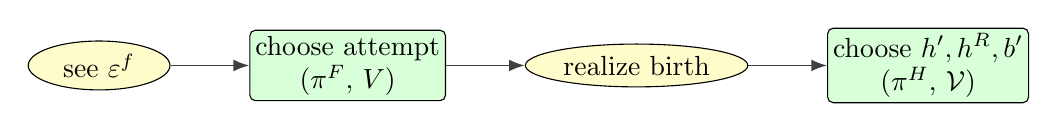
\begin{tikzpicture}[
  node distance=7mm and 10mm, >=Latex,
  see/.style={
    ellipse, draw, fill=yellow!20,
    minimum height=1.3em, minimum width=1.8cm,
    inner sep=2pt, align=center, font=\normalsize
  },
  choose/.style={
    rectangle, draw, fill=green!15, rounded corners=2pt,
    minimum height=1.5em, minimum width=1cm,
    inner sep=2pt, align=center, font=\normalsize
  },
  line/.style={-Latex, semithick, draw=black!75}
]
\node (fertS) [see, alt=<3>{draw=red, ultra thick}{}] {see $\varepsilon^f$};
\node (fertD) [choose, right=of fertS, alt=<3>{draw=red, ultra thick}{}] {choose attempt\\($\pi^F$, $V$)};
\node (succ) [see, right=of fertD, alt=<2>{draw=red, ultra thick}{}] {realize birth};
\node (house) [choose, right=of succ, alt=<2>{draw=red, ultra thick}{}] {choose $h',h^R,b'$\\($\pi^H$, $\mathcal V$)};

\draw[line] (fertS) -- (fertD);
\draw[line] (fertD) -- (succ);
\draw[line] (succ) -- (house);
\end{tikzpicture}%
}

\vspace{0.35em}
\raggedright
\setlength{\abovedisplayskip}{4pt}
\setlength{\belowdisplayskip}{4pt}

\only<1>{%
\small
\textbf{State.}
\[
x=(b,z,a,h,n,m),
\qquad
h\in\{0\}\cup\mathcal H^O.
\]

\begin{itemize}\setlength\itemsep{3pt}
  \item $b$: liquid wealth; $z$: earnings; $a$: age; $h$: inherited owner stock.
  \item $n$: parity; $m$: number of children currently at home.
  \item The model has one housing market, so location is suppressed.
\end{itemize}

\medskip
\textbf{Within the period:} observe the fertility shock, choose whether to attempt, realize conception success, then choose tenure, rooms, consumption, and saving.
}

\only<2>{%
\footnotesize
Conditional on the realized parity branch, the post-fertility value is
\[
\mathcal V_t(x)
=
\E_{\varepsilon_t^H}
\max_{h',h^R,b'}
\left\{
u_t(c,s;m)+\varepsilon_t^H(h')
+\beta s_a\E_t[V_{t+1}(x')]
+\beta(1-s_a)\mathcal B(w^e_{t+1})
\right\}.
\]

\begin{itemize}\setlength\itemsep{3pt}
  \item $h'h^R=0$: a renter sets $h'=0$; an owner sets $h^R=0$.
  \item Current purchases occur at $P_t$ and future sales at future prices.
  \item The budget, down-payment condition, and age-tapered debt floor restrict $(h',h^R,b')$.
  \item Household policies use the date-$(t+1)$ continuation value.
\end{itemize}
}

\only<3>{%
\footnotesize
Let $x^+$ add one birth, and let $\pi_a$ be conception success. Before the attempt taste shock:
\[
W_t^0(x)=\mathcal V_t(x),
\qquad
W_t^A(x)
=
\pi_a\!\left[
\mathcal V_t(x^+)-F_1\1\{n=0\}
\right]
+(1-\pi_a)\mathcal V_t(x).
\]
The attempt probability is
\[
\pi_t^F(x)
=
\frac{\exp\{W_t^A(x)/\kappa(n)\}}
{\exp\{W_t^A(x)/\kappa(n)\}+\exp\{W_t^0(x)/\kappa(n)\}},
\qquad
\kappa(n)=
\begin{cases}
\kappa_1,&n=0,\\
\kappa_C,&n\geq1.
\end{cases}
\]

\medskip
Housing affects fertility through current child-space needs, tenure feasibility, and the continuation value of wealth and housing.
}
\end{frame}

\begin{frame}{Persons, Heads, and Households}
The demographic block distinguishes three distributions:
\[
\underbrace{N_t}_{\text{resident persons}}
\quad\Longrightarrow\quad
\underbrace{H_t}_{\text{household heads}}
\quad\Longrightarrow\quad
\underbrace{G_t}_{\text{household economic states}}.
\]

\begin{itemize}\setlength\itemsep{0.65em}
  \item Births enter the person distribution immediately.
  \item Survival and migration move person cohorts across age and sex.
  \item Headship maps persons into the mass of household decision makers.
  \item The household transition moves wealth, earnings, tenure, parity, and child states within that head mass.
\end{itemize}

\vfill
The total mass of the household distribution must equal the head mass implied by persons.
\end{frame}

\begin{frame}{The Person-Cohort Law}
\small
Let $N_t^{g,a}$ denote resident persons of sex $g$ and single year of age $a$.

\medskip
The annual person law is
\[
N_{t+1}
=
A_{t+1}N_t+f_{t+1}B_{t+1}+M_{t+1}.
\]

\begin{itemize}\setlength\itemsep{0.5em}
  \item $A_{t+1}$ ages existing cohorts using destination-age survival.
  \item $f_{t+1}B_{t+1}$ allocates newborn survivors by sex at age zero.
  \item $M_{t+1}$ is the age--sex net-migration flow after survival.
  \item Model-period births are assigned to calendar cohorts before the annual law is iterated.
\end{itemize}

\vfill
Births and household heads remain distinct objects throughout the transition.
\end{frame}

\begin{frame}{The Household-Head Law}
\small
Fixed age--sex headship rates $\rho^{g,a}$ map persons into the target head stock:
\[
H_{t+1}^{g,a}
=
\rho^{g,a}N_{t+1}^{g,a}
=
H_{t+1}^{\mathrm{surv},g,a}
+F_{t+1}^{g,a}
-D_{t+1}^{g,a}
+H_{t+1}^{M,g,a}.
\]

The household operator supplies a raw within-age distribution
$\widetilde G_{t+1,a}$. Its mass is rescaled to the person-law head target:
\[
G_{t+1,a}(x)
=
H_{t+1,a}
\frac{\widetilde G_{t+1,a}(x)}
{\int\widetilde G_{t+1,a}(x')\,dx'}.
\]

\begin{itemize}\setlength\itemsep{0.4em}
  \item $F$ and $D$ are the minimum one-way formation or dissolution flow needed to attain $\rho^{g,a}$.
  \item Wealth, tenure, income, parity, and child-state composition are preserved within age.
  \item This is an accounting closure, not an estimated household-formation hazard.
\end{itemize}
\end{frame}

\begin{frame}{Transition Equilibrium}
A perfect-foresight transition is a path
\[
  \{V_t,\pi_t,G_t,N_t,H_t,P_t,r_t,T_t\}_{t=0}^{T}
\]
such that, at every date:
\begin{enumerate}\setlength\itemsep{0.55em}
  \item households optimize given future prices and transfers;
  \item births advance persons and heads, and the household distribution is rebalanced to head mass;
  \item occupied housing equals static-elastic supply;
  \item the asset-price/rent identity holds;
  \item property-tax revenue equals the equal transfer paid to household heads.
\end{enumerate}
\end{frame}

\begin{frame}{Steady-State Equilibrium}
A steady state is a constant tuple
\[
  (N^*,H^*,G^*,\pi^*,P^*,r^*,T^*)
\]
that satisfies simultaneously:
\begin{itemize}\setlength\itemsep{0.5em}
  \item household optimality and household-distribution stationarity;
  \item the person-cohort fixed point under the stated survival and migration closure;
  \item head formation and exact agreement between head mass and household mass;
  \item housing-market clearing, asset pricing, the government budget, and demographic reproduction.
\end{itemize}

\vfill
A finite path is not a steady state. Neither is a constant household distribution whose births fail to reproduce persons and heads.
\end{frame}

\begin{frame}{What the Quantitative Model Adds}
\small
\begin{itemize}\setlength\itemsep{0.6em}
  \item Sequential first and continuation births rather than a one-time family-size choice.
  \item A lifecycle of earnings, saving, tenure adjustment, child maturation, retirement, and death.
  \item A discrete owner ladder and continuous rental choice with collateral and transaction costs.
  \item Bequests and late-life housing retention.
  \item Separate laws for resident persons, household heads, and household economic states.
  \item Endogenous housing prices, rents, fiscal transfers, and demographic feedback.
\end{itemize}

\vfill
The quantitative model preserves the access mechanism while measuring its exposure and general-equilibrium consequences.
\end{frame}

\section{Quantification}

\begin{frame}[plain,c,noframenumbering]
\centering
{\Large\textbf{Quantification}}
\end{frame}

\begin{frame}{Dated Calibration}
The model is estimated at a point along the 2007--2023 transition.

\begin{enumerate}\setlength\itemsep{0.5em}
  \item Derive the 2007 fertility intercept so a constructed old benchmark has completed fertility 2.1.
  \item Reweight only the age marginal to the 2007 ACS household-head distribution.
  \item Estimate a linear fertility-preference change from 2007 through 2023.
  \item Impose Census household totals and ACS head-age shares at five dates.
  \item Match twelve moments, principally measured on the simulated 2023 state.
\end{enumerate}

\vfill
The household-total and age bridge is an input, not a fit. It is retired after 2023 and replaced by the person/head transition law.
\end{frame}

\begin{frame}{Externally Calibrated Parameters}
\small
\renewcommand{\arraystretch}{0.95}
\centering
\begin{tabular}{llcl}
\toprule
& \textbf{Param} & \textbf{Value} & \textbf{Source or restriction} \\
\midrule
\textit{Timing} & Model period & 4 years & Maintained \\
& Entry, maximum age & 18, 85 & Maintained \\
\midrule
\textit{Pref.} & $\sigma$ & 2.0 & Maintained \\
\midrule
\textit{Finance} & $\phi$ & 0.80 & 20\% buyer equity \\
& $\psi^s$ & 0.06 & Housing literature benchmark \\
\midrule
\textit{Housing} & Owner menu & $\{2,4,6,8,10\}$ & ACS rooms distribution \\
& Rental cap & 6 rooms & ACS rental distribution \\
& $\eta$ & 1.75 & Saiz benchmark \\
\midrule
\textit{Entry} & Wealth distribution & PSID & Childless renters, ages 18--24 \\
\bottomrule
\end{tabular}
\end{frame}

\begin{frame}{Internally Calibrated Parameters}
\footnotesize
\renewcommand{\arraystretch}{0.88}
\centering
\begin{tabular}{llc}
\toprule
\textbf{Param} & \textbf{Description} & \textbf{Estimate} \\
\midrule
$\beta_{\mathrm{annual}}$ & Annual discount factor & 0.994959 \\
$\kappa_1$ & First-birth logit scale & 2.267631 \\
$\kappa_C$ & Continuation-birth logit scale & 1.765427 \\
$\chi$ & Owner-service premium & 1.033945 \\
$H_0$ & Housing-supply scale & 16.381189 \\
$\theta_0$ & Bequest scale & 0.563219 \\
$\theta_1$ & Bequest wealth shift & 0.099707 \\
$h_m$ & Per-child room floor & 0.315267 \\
$h_1$ & First-child room jump & 0.199446 \\
$F_1$ & First-birth fixed cost & 4.545167 \\
$\Delta\psi_{2007:2023}$ & Fertility-preference change & $-0.350000$ \\
\bottomrule
\end{tabular}

\medskip
\small All eleven estimates are interior to their search bounds.
\end{frame}

\begin{frame}{Calibration Targets}
\fontsize{8.6}{10.0}\selectfont
\centering
\renewcommand{\arraystretch}{0.86}
\begin{tabular}{@{}llrr@{}}
\toprule
& \textbf{Moment} & \textbf{Target} & \textbf{Model} \\
\midrule
\textit{Fertility} & Completed fertility, women 40--44 & 1.918 & 1.918 \\
& Childless share, women 40--44 & 0.188 & 0.186 \\
& Mean age at first birth & 26.045 & 26.327 \\
& First births at age 30 or later & 0.260 & 0.242 \\
\midrule
\textit{Housing} & Four-year rooms contrast at first birth & 0.720 & 0.380 \\
& Rooms gap, 3+ versus 1--2 children & 0.368 & 0.359 \\
& Family ownership gap & 0.168 & 0.177 \\
& Ownership rate, ages 30--55 & 0.575 & 0.546 \\
& Mean occupied rooms, ages 18--85 & 5.780 & 6.710 \\
\midrule
\textit{Wealth} & Wealth / annual gross labor earnings & 6.873 & 6.766 \\
& Annual bequest flow / aggregate wealth & 0.0088 & 0.0086 \\
& Old wealth-to-income p90/p50 & 3.448 & 3.396 \\
\bottomrule
\end{tabular}
\end{frame}

\begin{frame}{Calibration Fit}
\centering
\includegraphics[width=0.92\textwidth,height=0.82\textheight,keepaspectratio]{../output/model/e5f_no_policy_transition_report_jump11_polish_r2_20260818/calibrated_2023_target_fit.pdf}
\end{frame}

\begin{frame}{What the Calibration Does Not Match}
\small
The strict SMM loss is $36.099$. Two housing moments account for $26.304$, or 73\% of the objective:
\[
\begin{array}{lrr}
\toprule
\text{Moment} & \text{Target} & \text{Model} \\
\midrule
\text{Four-year rooms contrast at first birth} & 0.720 & 0.380 \\
\text{Mean occupied rooms} & 5.780 & 6.710 \\
\bottomrule
\end{array}
\]

\begin{itemize}\setlength\itemsep{0.45em}
  \item Fertility stocks, tenure, and wealth fit more closely than housing quantities.
  \item The weighted Jacobian has rank $10/11$ at the predeclared $10^{-3}$ threshold.
  \item Its condition number is $1{,}104$; the weakest direction loads primarily on the bequest shift $\theta_1$.
  \item The estimate is reproducible and interior, but locally weakly identified and not a claim of global optimality.
\end{itemize}
\end{frame}

\begin{frame}{From the 2023 Fit to the Transition}
\small
\begin{table}
\centering
\begin{tabular}{@{}lccp{0.36\textwidth}@{}}
\toprule
Object & Annual tax & Rebate & Role \\
\midrule
Calibration status quo & 1\% & None & Fitted 2023 reference \\
Transition reference & 1\% & Equal per head & Accepted forward path \\
Policy counterfactual & 2\% & Equal per head & Same equilibrium closure \\
\bottomrule
\end{tabular}
\end{table}

\medskip
The accepted transition begins from:
\[
\text{338.7 million persons},
\qquad
\text{129.0 million heads},
\qquad
\text{the fitted 2023 household state}.
\]

Supply is reanchored so the rebated 1\% economy clears at the inherited quantity.
The transition reference is rebated; it is not the unrebated calibration status quo.
\end{frame}

\begin{frame}{Demographic Momentum}
\centering
\includegraphics[width=0.98\textwidth,trim=0 470bp 0 0,clip]{\baselinefigure}

\vspace{0.15em}
\small
Resident persons rise from 338.7 million in 2023 to 344.6 million in 2039.
Household heads peak in 2047 at 142.1 million. Both stocks then contract toward
the conditional terminal equilibrium.

\medskip
An inherited age distribution generates decades of momentum even when subsequent births are low.
\end{frame}

\begin{frame}{Prices and Births Move on Different Clocks}
\centering
\includegraphics[width=0.98\textwidth,trim=0 232bp 0 255bp,clip]{\baselinefigure}

\vspace{0.1em}
\small
The asset price peaks in 2055. The renter price peaks in 2083 because it also
reflects the next-period asset payoff. Annual births per head undershoot their
terminal rate before converging back toward it.

\medskip
Cohort composition, forward-looking capitalization, and household fertility need not turn at the same date.
\end{frame}

\begin{frame}{The Conditional Terminal Equilibrium}
\small
\begin{table}
\centering
\begin{tabular}{@{}lrrr@{}}
\toprule
Object & 2023 & Terminal & Change \\
\midrule
Resident persons, millions & 338.724 & 184.278 & $-45.6\%$ \\
Household heads, millions & 128.964 & 76.073 & $-41.0\%$ \\
Asset price & 0.6229 & 0.4977 & $-20.1\%$ \\
Rent-equivalent price & 0.0936 & 0.0825 & $-11.8\%$ \\
Annual births per head & 0.02152 & 0.01699 & $-21.0\%$ \\
\bottomrule
\end{tabular}
\end{table}

\medskip
The terminal demographic renewal ratio is $0.5568$. A constant positive
population is sustained by the fixed age--sex migration flow.

\vfill
This is a conditional fixed-migration equilibrium, not a forecast of the U.S.\ population level.
\end{frame}

\begin{frame}{The Rebated Property Tax}
The reform permanently raises the annual property-tax rate from 1\% to 2\%
and returns all contemporaneous revenue equally across household heads:
\[
T_t\int dG_t
=
\tau_{H,t}P_tQ_t^H,
\qquad
Q_t^H=\int h_t(x)\,dG_t(x).
\]

\begin{itemize}\setlength\itemsep{0.5em}
  \item \textbf{Capitalization}: a higher carrying cost tends to reduce the asset price.
  \item \textbf{User cost}: the renter price depends on the tax and the next asset price.
  \item \textbf{Tenure and fertility}: down payments, owner products, and child-space choices adjust state by state.
  \item \textbf{Demographic scale}: changed births affect persons now and household heads only later.
\end{itemize}

\vfill
All effects are general equilibrium: prices, tenure, births, population, and the per-head rebate evolve together.
\end{frame}

% Add a quantitative 2%-minus-1% result frame only from an accepted comparison packet.

\begin{frame}{Conclusion}
\small
\begin{itemize}\setlength\itemsep{0.7em}
  \item Children raise demand for rooms; rental size and down payments determine access to that space.
  \item Fertility, tenure, saving, and old-age housing retention must be solved jointly over the lifecycle.
  \item Births create persons; survival, migration, and head formation create household heads.
  \item The calibrated model fits fertility stocks, tenure, and wealth more closely than housing quantities.
  \item The accepted transition displays demographic momentum followed by slow convergence to a conditional fixed-migration equilibrium.
\end{itemize}

\vfill
{\normalsize\textbf{Housing policy can affect family formation today and housing demand generations later.}}
\end{frame}

\begin{frame}[plain,c,noframenumbering]
\centering
{\Large\textbf{Thank You}}
\end{frame}

% ============================================================================
% APPENDIX
% ============================================================================

\appendix

\begin{frame}[plain,noframenumbering]
\centering
\vfill
{\Large\textbf{Appendix}}
\vfill
\end{frame}

% Supporting theory: original household problems and the dated allocation results.
\begin{frame}[label=theory-young-problems]{Young Household Problems}
\relax
\small\linespread{1.05}\selectfont
\setlength{\abovedisplayskip}{4pt}
\setlength{\belowdisplayskip}{4pt}
\setlength{\abovedisplayshortskip}{4pt}
\setlength{\belowdisplayshortskip}{4pt}
{\small A prime denotes next-period net financial wealth. Taking prices and rebates as given:}
{\small
\small\linespread{1.05}\selectfont
\setlength{\abovedisplayskip}{4pt}
\setlength{\belowdisplayskip}{4pt}
\setlength{\abovedisplayshortskip}{4pt}
\setlength{\belowdisplayshortskip}{4pt}
\[
\begin{aligned}
W_t^R(i)&=\max_{c,h,n,a'}\ u_t^y(c,h,n)+\beta V_{t+1}^R(a';i),\\
&c+qa'+qr_t h=y_i^y+b_i+T_t,\quad a'\ge0,\quad h\le h_R^{\max},\\[0.6em]
W_t^O(i)&=\max_{c,h,n,a'}\ u_t^y(c,h,n)+\beta V_{t+1}^O(a',h;i),\\
&c+qa'+(1+q\tau_t^p)P_t h=y_i^y+b_i+T_t,\\
&qa'+\phi_tP_t h\ge0,\qquad h\le h_O^{\max}.
\end{aligned}
\]
}
{\small Mortgage principal $d$ and current bond investment $k$ satisfy $0\le d\le\phi_tP_t h$, $k\ge0$, and $a'=(k-d)/q$. Thus a buyer supplies at least the down payment $(1-\phi_t)P_t h$.\par}
\medskip
{\small Current income, wealth and the rebate are available at purchase. Utility requires $c>\chi n$, $h>\kappa n$, and $n>0$.\par}
\vfill
\hyperlink{theory-households}{\beamerbutton{Back}}\quad\hyperlink{theory-old-problems}{\beamerbutton{Old households}}
\end{frame}

\begin{frame}[label=theory-old-problems]{Old Households and Estates}
\relax
\small\linespread{1.05}\selectfont
\setlength{\abovedisplayskip}{4pt}
\setlength{\belowdisplayskip}{4pt}
\setlength{\abovedisplayshortskip}{4pt}
\setlength{\belowdisplayshortskip}{4pt}
{\small An old owner has net financial wealth $a$ and inherited housing $H$. Old households solve:}
{\small
\small\linespread{1.05}\selectfont
\setlength{\abovedisplayskip}{4pt}
\setlength{\belowdisplayskip}{4pt}
\setlength{\abovedisplayshortskip}{4pt}
\setlength{\belowdisplayshortskip}{4pt}
\setlength{\abovedisplayskip}{4pt}\setlength{\belowdisplayskip}{4pt}
\[
\begin{aligned}
V_t^R(a;i)&=\max_{c^o,h^o,e}\ u^o(c^o,h^o,e),\\
&c^o+qe+qr_t h^o=a+y_i^o+T_t,\quad h^o\le h_R^{\max},\\[0.45em]
V_t^O(a,H;i)&=\max_{c^o,h^o,e}\ u^o(c^o,h^o,e),\\
&c^o+qe+qr_t h^o=a+P_tH+y_i^o+T_t,\\
&h^o\le h_O^{\max},\qquad e\ge P_{t+1}h^o.
\end{aligned}
\]
}
{\small Owners can sell and resize. With financial saving $a^e\ge0$, the estate paid at death is:}
\[
e=\begin{cases}a^e/q,&\text{renter},\\ a^e/q+P_{t+1}h^o,&\text{owner}.\end{cases}
\]
{\small The owner's estate floor is equivalent to nonnegative financial saving. The estate enters the parent's utility; entry wealth is exogenous.\par}
\vfill
\hyperlink{theory-households}{\beamerbutton{Back}}
\end{frame}

\begin{frame}[label=theory-planner-solution]{The Planner's Solution}
\relax
\small\linespread{1.05}\selectfont
\setlength{\abovedisplayskip}{4pt}
\setlength{\belowdisplayskip}{4pt}
\setlength{\abovedisplayshortskip}{4pt}
\setlength{\belowdisplayshortskip}{4pt}
{\small Write $\bar x=\int(c_i^{y,eq}-\chi n_i)\,\mathrm dQ$ and $\bar s=\int(h_i^{y,eq}-\kappa n_i)\,\mathrm dQ$. For each household let $H_i=h_{d_i}^{\max}$. The optimal allocation is:}
{\small
\small\linespread{1.05}\selectfont
\setlength{\abovedisplayskip}{4pt}
\setlength{\belowdisplayskip}{4pt}
\setlength{\abovedisplayshortskip}{4pt}
\setlength{\belowdisplayshortskip}{4pt}
\[
\begin{aligned}
c_i^{y,F}&=\chi n_i+\tfrac12(\bar x+\bar c^{o,eq}),&
c_i^{o,F}&=\tfrac12(\bar x+\bar c^{o,eq}),\\[0.4em]
h_i^{y,F}&=\min\{H_i,\kappa n_i+\alpha/\lambda_H\},&
h_i^{o,F}&=\min\{H_i,\gamma/\lambda_H\}.
\end{aligned}
\]
}
{\small Adult consumption is equalized; $\lambda_H$ clears the housing market. Below size limits, marginal housing utility is equalized.\par}
\medskip
{\small Binding planner limits still permit an aggregate young housing gain if:}
{\small
\small\linespread{1.05}\selectfont
\setlength{\abovedisplayskip}{4pt}
\setlength{\belowdisplayskip}{4pt}
\setlength{\abovedisplayshortskip}{4pt}
\setlength{\belowdisplayshortskip}{4pt}
\[
\bar h^{o,eq}>\frac\gamma\alpha\bar s,\qquad
H_i-\kappa n_i\ge\bar s\ \text{for all }i,\qquad
Q\{H_i-\kappa n_i>\bar s\}>0.
\]
}
{\small Every household can accommodate its children and the reference mean adult space, with some capacity beyond that amount.\par}
\vfill
{\footnotesize This is an equally weighted allocation comparison. A difference from it does not by itself establish a Pareto improvement.\hfill\hyperlink{theory-allocation}{\beamerbutton{Back}}\par}
\end{frame}

\begin{frame}[label=theory-primitives]{An Income Condition}
\relax
\small\linespread{1.05}\selectfont
\setlength{\abovedisplayskip}{4pt}
\setlength{\belowdisplayskip}{4pt}
\setlength{\abovedisplayshortskip}{4pt}
\setlength{\belowdisplayshortskip}{4pt}
{\small Set $\phi=q$ and $\tau^p=0$. Let $w_i=y_i^y+b_i$, $v_i=y_i^o$, $E=1+\alpha+\vartheta$, and $K=1+\gamma+\omega_B$. With endowments on compact, strictly positive support, suppose:}
{\small
\small\linespread{1.05}\selectfont
\setlength{\abovedisplayskip}{4pt}
\setlength{\belowdisplayskip}{4pt}
\setlength{\abovedisplayshortskip}{4pt}
\setlength{\belowdisplayshortskip}{4pt}
\[
\omega_B(1-q)>q\gamma,\qquad
\frac{v_i}{w_i}>\frac{\beta K}{qE}\ \text{for all }i,\qquad
\frac{\nu\vartheta\bar w}{E}>\chi.
\]
}
{\small With competitive choices below both size limits, the stationary allocation is:}
{\small
\small\linespread{1.05}\selectfont
\setlength{\abovedisplayskip}{4pt}
\setlength{\belowdisplayskip}{4pt}
\setlength{\abovedisplayshortskip}{4pt}
\setlength{\belowdisplayshortskip}{4pt}
\[
\begin{aligned}
p&=\frac{\nu\vartheta\bar w/E-\chi}{\kappa},&P&=\frac p{1-q},\\
x_i&=\frac{w_i}{E},&n_i&=\frac{w_i}{\nu\bar w},\\
h_i^y&=\frac{\alpha w_i}{Ep}+\frac{\kappa w_i}{\nu\bar w},&
c_i^o&=\frac{v_i}{K},\quad h_i^o=\frac{\gamma v_i}{Kp}.
\end{aligned}
\]
}
{\small The fixed-fertility planner raises young housing, and the joint planner raises fertility, if:}
\[
\frac{\bar v}{K}>\frac{\bar w}{E}.
\]
{\footnotesize Future income cannot be fully brought forward. This condition allows $\beta R_f$ on either side of one.\hfill\hyperlink{theory-regime-checks}{\beamerbutton{Size limits}}\quad\hyperlink{theory-allocation}{\beamerbutton{Back}}\par}
\end{frame}

\begin{frame}[label=theory-regime-checks]{Financing and Size Limits}
\relax
\small\linespread{1.05}\selectfont
\setlength{\abovedisplayskip}{4pt}
\setlength{\belowdisplayskip}{4pt}
\setlength{\abovedisplayshortskip}{4pt}
\setlength{\belowdisplayshortskip}{4pt}
{\small In the preceding income benchmark, housing services cost $p=(1-q)P$. Old households with resources $z$ choose:}
\[
c^o=\frac zK,\qquad h^o=\frac{\gamma z}{Kp},\qquad e=\frac{\omega_Bz}{Kq}.
\]
{\small The estate condition makes owner financial saving positive. With $\phi=q$, the constrained young enter old age with $z=v_i$ and have financing multiplier:}
\[
\mu_i=\frac E{w_i}-\frac{\beta K}{qv_i}>0.
\]
{\small An explicit sufficient bound keeps competitive and planner housing choices below their limits:}
\[
\frac{\alpha w_{\max}}{Ep}+\frac{\kappa w_{\max}}{\nu\bar w}
+\frac{\gamma v_{\max}}{Kp}
<h_R^{\max}<h_O^{\max}.
\]
{\small This benchmark has both tenures, but their real choices coincide and rental size limits are inactive. At $\phi=q$, the house's sale value exactly repays a constrained owner's mortgage.\par}
\vfill
\hyperlink{theory-primitives}{\beamerbutton{Back}}
\end{frame}

\begin{frame}[label=theory-fertility-proof]{Private Fertility after Reallocation}
\relax
\small\linespread{1.05}\selectfont
\setlength{\abovedisplayskip}{4pt}
\setlength{\belowdisplayskip}{4pt}
\setlength{\abovedisplayshortskip}{4pt}
\setlength{\belowdisplayshortskip}{4pt}
{\small Let $x=c-\chi n$ and $s=h-\kappa n$. Differentiating the parent's fertility condition gives:}
\[
\mathrm dn=
\frac{\chi\,\mathrm dc/x^2+\alpha\kappa\,\mathrm dh/s^2}
{\vartheta/n^2+\chi^2/x^2+\alpha\kappa^2/s^2}.
\]
{\small The denominator is positive. More housing and weakly more consumption raise fertility.\par}
\medskip
{\small For a finite housing gain $\Delta h\ge0$ and consumption loss $\Delta c=-d\le0$, if the original fertility remains feasible:}
\[
n_1\ge n_0
\quad\Longleftrightarrow\quad
d\le
\frac{\alpha\kappa x^2\Delta h}
{\chi s(s+\Delta h)+\alpha\kappa x\Delta h}.
\]
{\small The admissible loss of consumption depends on how scarce goods and space were initially. These are household comparisons at given bundles.\par}
\vfill
\hyperlink{theory-fertility}{\beamerbutton{Back}}
\end{frame}

\begin{frame}[label=theory-joint-fertility]{Fertility Chosen by the Planner}
\relax
\small\linespread{1.05}\selectfont
\setlength{\abovedisplayskip}{4pt}
\setlength{\belowdisplayskip}{4pt}
\setlength{\abovedisplayshortskip}{4pt}
\setlength{\belowdisplayshortskip}{4pt}
{\small Let the same dated planner also choose $n_i$, valuing children through parents' utility. With slack size limits, common fertility $n^J$ satisfies:}
\[
\frac\vartheta{n^J}
=\frac{2\chi}{C^{eq}/N-\chi n^J}
+\frac{\kappa(\alpha+\gamma)}{\bar H/N-\kappa n^J}.
\]
{\small Consumption and housing adjust jointly with fertility; children's resource needs enter once.\par}
\medskip
{\small With $\bar x=\overline{c^{y,eq}-\chi n}$ and $\bar s=\overline{h^{y,eq}-\kappa n}$, sufficient conditions for higher mean fertility and young housing are:}
\[
\bar c^{o,eq}\ge\bar x,\qquad
\bar h^{o,eq}\ge\frac\gamma\alpha\bar s,\qquad
h_R^{\max}>\bar h^{y,eq},
\]
{\small with at least one of the first two inequalities strict. Planner size limits may bind.\par}
\vfill
{\footnotesize This joint choice differs from parents rechoosing fertility after a fixed-fertility allocation; mean fertility in that second experiment can fall.\hfill\hyperlink{theory-fertility}{\beamerbutton{Back}}\par}
\end{frame}

\begin{frame}[label=theory-transition-conditions]{Conditions for the Local Transition}
\relax
\small\linespread{1.05}\selectfont
\setlength{\abovedisplayskip}{4pt}
\setlength{\belowdisplayskip}{4pt}
\setlength{\abovedisplayshortskip}{4pt}
\setlength{\belowdisplayshortskip}{4pt}
{\footnotesize Use the stationary income benchmark: $\phi=q$, zero reference tax, uniformly strict young finance, housing-cap and old financial-estate margins on the compact endowment support. Let $W=\bar w$, $V=\bar v$, and $\pi=\operatorname{logistic}(\bar\xi/\sigma_\xi)$. Define:}
{\small
\small\linespread{1.05}\selectfont
\setlength{\abovedisplayskip}{4pt}
\setlength{\belowdisplayskip}{4pt}
\setlength{\abovedisplayshortskip}{4pt}
\setlength{\belowdisplayshortskip}{4pt}
\[
\epsilon=\frac{p\kappa}{\chi+p\kappa},\qquad
A=\alpha+\vartheta\epsilon,\qquad
\zeta=\frac{\gamma EV}{KWA},
\quad E=1+\alpha+\vartheta,\ K=1+\gamma+\omega_B.
\]
}
{\small Sufficient restrictions are:}
{\small
\small\linespread{1.05}\selectfont
\setlength{\abovedisplayskip}{4pt}
\setlength{\belowdisplayskip}{4pt}
\setlength{\abovedisplayshortskip}{4pt}
\setlength{\belowdisplayshortskip}{4pt}
\[
\begin{gathered}
V\ge W,\qquad
\frac\alpha{1+\alpha}<\epsilon<q,\qquad
1<\zeta<\frac{2E\epsilon}{A}-1,\\[0.3em]
\omega_B(1-q)>q\gamma,\qquad
\frac{\pi\gamma}{K}<\min\{(1-q)^2,q\zeta\}.
\end{gathered}
\]
}
{\small Sufficiently small permanent taste and tax changes have unique local bounded perfect-foresight paths converging to their stationary equilibria. The tax is unexpected when introduced along the baseline path.\par}
\vfill
{\footnotesize The result is local to this constraint regime. Later fertility differences may change sign.\hfill\hyperlink{theory-transition}{\beamerbutton{Back}}\par}
\end{frame}

\begin{frame}[label=theory-transition-curves]{Fertility and Terminal Population}
\relax
\small\linespread{1.05}\selectfont
\setlength{\abovedisplayskip}{4pt}
\setlength{\belowdisplayskip}{4pt}
\setlength{\abovedisplayshortskip}{4pt}
\setlength{\belowdisplayshortskip}{4pt}
{\small Starting from the same young cohort, demographic accounting gives:}
\[
\frac{Y_T^{\rm policy}}{Y_T^{\rm baseline}}
=\prod_{t=t_p}^{T-1}\frac{\bar n_t^{\rm policy}}{\bar n_t^{\rm baseline}}.
\]
{\small Under the local transition conditions, the permanent rebated tax raises fertility on impact and the terminal cohort mass from $N_0$ to $N_1>N_0$:}
\[
\sum_{t=t_p}^{\infty}\log
\frac{\bar n_t^{\rm policy}}{\bar n_t^{\rm baseline}}
=\log\frac{N_1}{N_0}>0,
\qquad \bar n_0^*=\bar n_1^*=1/\nu.
\]
{\small Terminal adult households are $2N$. The population difference reflects cumulative fertility along the transition.\par}
\medskip
{\small The policy need not implement the planner's allocation. Across stationary tax equilibria, mean young housing falls with the rebate even as total young housing rises:}
\[
\frac{\mathrm d\bar h^y}{\mathrm dT}
=-\frac{\alpha\chi}{E\kappa p^2}<0.
\]
\vfill
\hyperlink{theory-transition}{\beamerbutton{Back}}
\end{frame}

\begin{frame}{Bellman Timing}
Within a four-year date, the household:
\begin{enumerate}
  \item observes fertility taste shocks and, when eligible, chooses whether to wait or attempt a birth;
  \item realizes conception success and chooses renter rooms or an owner product conditional on parity;
  \item chooses consumption and next-period liquid wealth;
  \item receives income and pays rent, property tax, depreciation, and any moving cost;
  \item ages children independently, transitions income, and survives or leaves a warm-glow estate.
\end{enumerate}

In a transition, date-$t$ policies use the date-$(t+1)$ continuation value.
The terminal value function and next-date asset price are boundary conditions;
they do not replace convergence of the simulated terminal distribution.
\end{frame}

\begin{frame}{Exact Annual Person Accounting}
The annual law can be written cell by cell. For newborns,
\[
N_{t+1}^{g,0}
=
s_{t+1}^{g,0}f_{t+1}^{g}B_{t+1}
+
M_{t+1}^{g,0}.
\]
For interior ages $a\geq1$,
\[
N_{t+1}^{g,a}
=
s_{t+1}^{g,a}N_t^{g,a-1}
+
M_{t+1}^{g,a}.
\]
The terminal age is top coded, so survivors from the penultimate and terminal
cells both enter the last cell. Every step satisfies
\[
\sum N_{t+1}
=
\sum N_t+B_{t+1}
-\text{newborn deaths}
-\text{existing deaths}
+\sum M_{t+1}.
\]
\end{frame}

\begin{frame}{Exact Household-Head Accounting}
Surviving heads are aged with the same survival schedule. In each cell, the
target is $\rho^{g,a}N_{t+1}^{g,a}$. The accounting closure uses only one
gross adjustment direction:
\[
F_{t+1}^{g,a}
=
\max\left\{
\rho^{g,a}N_{t+1}^{\mathrm{preM},g,a}
-H_{t+1}^{\mathrm{surv},g,a},0
\right\},
\]
\[
D_{t+1}^{g,a}
=
\max\left\{
H_{t+1}^{\mathrm{surv},g,a}
-\rho^{g,a}N_{t+1}^{\mathrm{preM},g,a},0
\right\},
\qquad
H_{t+1}^{M,g,a}
=
\rho^{g,a}M_{t+1}^{g,a}.
\]
Hence $H_{t+1}^{g,a}=\rho^{g,a}N_{t+1}^{g,a}$ exactly. Formation and
dissolution are accounting flows, not simultaneous estimated hazards.
\end{frame}

\begin{frame}{The Within-Age Household Bridge}
Let $\widetilde G_{t+1,a}(x)$ be the raw household transition within age $a$,
and let $H_{t+1,a}$ be the head mass implied by persons. Then
\[
G_{t+1,a}(x)
=
\begin{cases}
\displaystyle
H_{t+1,a}
\frac{\widetilde G_{t+1,a}(x)}
{\int\widetilde G_{t+1,a}(x')\,dx'},
&
\int\widetilde G_{t+1,a}>0,
\\[1.2em]
H_{t+1,a}\Gamma_a(x),
&
\text{for an empty entrant age cell},
\end{cases}
\]
where $\Gamma_a$ is the externally specified entrant template. The operation
exposes added and removed mass separately and moves no mass across ages.

A richer model would estimate economic states for newly formed, dissolved,
and migrant heads rather than preserve the raw conditional composition.
\end{frame}

\begin{frame}{Steady-State Demographic Scale}
With fixed terminal survival $A$, newborn-survivor vector $f$, net migration
$m$, and headship vector $\rho$, persons satisfy
\[
N^*
=
AN^*+f\,b^*(\rho'N^*)+m,
\]
where $b^*$ is annual births per head implied by household policy.

\medskip
Define
\[
v_B=(I-A)^{-1}f,
\qquad
v_M=(I-A)^{-1}m.
\]
The demographic renewal ratio is
\[
\mathcal R=b^*\rho'v_B.
\]
When fixed migration is positive, a finite steady state requires
$\mathcal R<1$, and
\[
B^*=\frac{b^*\rho'v_M}{1-\mathcal R},
\qquad
N^*=v_M+B^*v_B.
\]
\end{frame}

\begin{frame}{Market and Fiscal Closure}
At every date, occupied physical rooms satisfy
\[
\int h(x;\pi_t)\,dG_t(x)
=
H_{2023}
\left(\frac{P_t}{P_{2023}}\right)^\eta.
\]
The rebated tax satisfies
\[
\tau_{H,t}P_tQ_t^H
=
T_t\int dG_t.
\]
At a stationary price,
\[
r^*
=
(R_b-1+\delta_H+\tau_H)P^*.
\]

Housing demand uses physical rooms. The owner-service premium affects utility
but does not create additional physical supply. Conditional renter housing is
also distinct from realized housing after the tenure choice.
\end{frame}

\begin{frame}{Complete Target Fit I}
\centering
\tiny
\setlength{\tabcolsep}{3.2pt}
\begin{tabularx}{\textwidth}{@{}Yrrrrr@{}}
\toprule
Moment & Target & Model & Gap & Weight & Loss \\
\midrule
Completed fertility, women 40--44 & 1.918000 & 1.918251 & 0.000251 & 1,425.739 & 0.000090 \\
Childless share, women 40--44 & 0.188000 & 0.185867 & $-0.002133$ & 17,180.744 & 0.078133 \\
Mean age at first birth & 26.044627 & 26.327334 & 0.282707 & 44.444 & 3.552148 \\
First births at age 30 or later & 0.260327 & 0.242115 & $-0.018213$ & 10,000.000 & 3.316971 \\
Four-year rooms contrast at first birth & 0.720246 & 0.379786 & $-0.340461$ & 137.565 & 15.945664 \\
Rooms gap, 3+ versus 1--2 children & 0.367700 & 0.359253 & $-0.008447$ & 2,958.515 & 0.211071 \\
\bottomrule
\end{tabularx}

\vspace{0.7em}
\small
Completed fertility and childlessness are CPS age-42 cohort stocks. First-birth
timing uses a fixed synthetic cohort. The rooms response follows the 2019
childless risk set through matched birth and no-birth branches to 2023.
\end{frame}

\begin{frame}{Complete Target Fit II}
\centering
\tiny
\setlength{\tabcolsep}{3.2pt}
\begin{tabularx}{\textwidth}{@{}Yrrrrr@{}}
\toprule
Moment & Target & Model & Gap & Weight & Loss \\
\midrule
Family ownership gap & 0.167662 & 0.176866 & 0.009204 & 14,229.591 & 1.205562 \\
Ownership rate, ages 30--55 & 0.575472 & 0.546060 & $-0.029412$ & 1,207.846 & 1.044837 \\
Mean occupied rooms, ages 18--85 & 5.779970 & 6.710105 & 0.930135 & 11.973 & 10.358582 \\
Wealth / annual gross labor earnings & 6.873100 & 6.766352 & $-0.106748$ & 6.288 & 0.071648 \\
Annual bequest flow / aggregate wealth & 0.008800 & 0.008623 & $-0.000177$ & 5,165,289.256 & 0.161538 \\
Old wealth-to-income p90/p50 & 3.448111 & 3.396287 & $-0.051824$ & 56.960 & 0.152979 \\
\midrule
\multicolumn{5}{r}{\textbf{Total strict loss}} & \textbf{36.099223} \\
\bottomrule
\end{tabularx}

\vspace{0.7em}
\small
All twelve moments enter the same active objective. The first-birth rooms row
is retained as a descriptive contrast despite its non-flat prepath.
\end{frame}

\begin{frame}{Free Parameters I}
\centering
\scriptsize
\begin{tabularx}{\textwidth}{@{}p{0.22\textwidth}Yrr@{}}
\toprule
Parameter & Economic interpretation & Estimate & Search bound \\
\midrule
$\beta_{\mathrm{annual}}$ & Patience & 0.994959 & $[0.9400,0.9995]$ \\
$\kappa_1$ & First-birth logit scale & 2.267631 & $[0.02,50]$ \\
$\kappa_C$ & Continuation-birth logit scale & 1.765427 & $[0.02,50]$ \\
$\chi$ & Owner-service premium & 1.033945 & $[0.10,5]$ \\
$H_0$ & Housing-supply scale & 16.381189 & $[0.20,80]$ \\
$\theta_0$ & Bequest scale & 0.563219 & $[0,8]$ \\
\bottomrule
\end{tabularx}

\vspace{0.5em}
No estimate is within two percent of its transformed search boundary.
\end{frame}

\begin{frame}{Free Parameters II}
\centering
\scriptsize
\begin{tabularx}{\textwidth}{@{}p{0.22\textwidth}Yrr@{}}
\toprule
Parameter & Economic interpretation & Estimate & Search bound \\
\midrule
$\theta_1$ & Bequest wealth shift & 0.099707 & $[0.02,16]$ \\
$h_m$ & Per-child room floor & 0.315267 & $[0.10,1.80]$ \\
$h_1$ & First-child room jump & 0.199446 & $[0,0.50]$ \\
$F_1$ & First-birth fixed cost & 4.545167 & $[0,8]$ \\
$\Delta\psi_{2007:2023}$ & Fertility-preference change & $-0.350000$ & $[-1.50,0.20]$ \\
\bottomrule
\end{tabularx}

\vspace{0.6em}
The implied fertility intercepts are $\psi_{2007}=0.280341$ and
$\psi_{2023}=-0.069659$. The intercept change is a reduced-form residual, not
a causally identified preference shock.
\end{frame}

\begin{frame}{Assigned Household and Market Objects}
\centering
\scriptsize
\begin{tabularx}{0.97\textwidth}{@{}p{0.28\textwidth}p{0.20\textwidth}Y@{}}
\toprule
Parameter & Value & Source or restriction \\
\midrule
Model period & 4 years & Timing \\
Entry and maximum ages & 18 and 85 & Timing \\
Risk aversion $\sigma$ & 2 & Maintained \\
Financed share $\phi$ & 0.80 & 20\% buyer-equity restriction \\
Sale cost & 6\% & Housing literature benchmark \\
Owner room menu & $\{2,4,6,8,10\}$ & ACS occupied-room distribution \\
Rental cap & 6 rooms & ACS rental-size distribution \\
Supply elasticity $\eta$ & 1.75 & Saiz benchmark \\
Entrant wealth & PSID ratio distribution & Childless renters age 18--24 \\
Tenure taste-shock scale & 0 & Author restriction \\
Child dependence of bequests & 0 & Child-invariant warm glow \\
\bottomrule
\end{tabularx}
\end{frame}

\begin{frame}{Historical Calibration Bridge}
The 2007--2023 calibration uses five four-year dates. At each date, the
observed household total and head-age marginal are imposed before the twelve
maintained moments are evaluated.

\begin{itemize}
  \item This absorbs household formation and migration that births since 2007 cannot generate by 2023.
  \item It makes the cross-section a dated state rather than a stationary distribution.
  \item Historical fertility, ownership, rooms, and price paths are holdouts unless explicitly included in the target system.
  \item The bridge is retired after 2023 and replaced by the person/head law.
\end{itemize}

Matching the imposed population path is an accounting identity, not evidence
that the model explains U.S.\ household growth over 2007--2023.
\end{frame}

\begin{frame}{Local Identification Audit}
\small
At the selected vector, the standardized residual is
\[
r_j(\theta)
=
\sqrt{w_j}\,[m_j(\theta)-\widehat m_j].
\]
A fresh two-sided coordinate panel constructs the weighted Jacobian
$J=\partial r/\partial\theta$.

\begin{table}
\centering
\footnotesize
\begin{tabularx}{0.96\textwidth}{@{}Yrr@{}}
\toprule
Jacobian & Rank at $10^{-3}$ & Condition number \\
\midrule
All 11 free parameters & 10/11 & 1,104.01 \\
Ten active columns after freezing the inconsistent bequest column & 10/10 & 391.02 \\
\bottomrule
\end{tabularx}
\end{table}

The weakest right-singular vector places 91.9\% of its absolute loading on
$\theta_1$. Local weak identification is concentrated in the bequest block.
\end{frame}

\begin{frame}{Accepted Baseline Equilibrium Checks}
\begin{table}
\centering
\footnotesize
\begin{tabularx}{0.94\textwidth}{@{}p{0.22\textwidth}p{0.23\textwidth}Y@{}}
\toprule
Object & Max. absolute residual & Interpretation \\
\midrule
Housing market & $1.7943\times10^{-4}$ & Demand relative to supply \\
Fiscal budget & $1.1572\times10^{-5}$ & Revenue minus equal transfers \\
Person identity & numerical precision & Births, deaths, and migration \\
Head identity & numerical precision & Deaths, formation, dissolution, migrant heads \\
Household/head identity & numerical precision & Household mass equals person-law head mass \\
\bottomrule
\end{tabularx}
\end{table}

\vspace{0.3em}
\small
The final endogenous date is also close to the independently solved terminal
person distribution, head distribution, household distribution, price, rent,
transfer, and fertility preference.
\end{frame}

\begin{frame}{Slow Terminal Convergence}
The dominant eigenvalue of the frozen-terminal four-year demographic block is
\[
\lambda_1=0.960754.
\]
It implies
\[
\text{half-life}
=
\frac{4\log(1/2)}{\log\lambda_1}
\approx69\ \text{years},
\qquad
\lambda_1^{116}<0.01.
\]

Thus one-percent attenuation of the slow mode requires about 116 model periods,
or 464 years. The accepted path uses 128 four-year periods so the simulated
state approaches the terminal fixed point rather than merely inheriting it as
a boundary condition.

\vfill
The long horizon reflects age-structured demographic persistence, not a forecast horizon.
\end{frame}

\begin{frame}{Baseline Transition Diagnostics}
\centering
\includegraphics[width=0.98\textwidth,trim=0 0 0 488bp,clip]{\baselinefigure}

\vspace{0.1em}
\small
The equal rebate and equilibrium residuals are solved jointly with prices.
The displayed residuals remain below their common acceptance thresholds
throughout the path.
\end{frame}

\begin{frame}{Policy Comparison Contract}
A quantitative 2\%--minus--1\% comparison must hold fixed:
\begin{itemize}
  \item the fitted 2023 household state and reconstructed person/head stocks;
  \item survival, net migration, birth sex shares, and headship;
  \item the housing-supply elasticity and 2023 supply anchor;
  \item the terminal fertility preference and all calibrated household parameters;
  \item the equal-rebate rule and the definitions of housing and fiscal residuals.
\end{itemize}

The comparison then separates the immediate response of prices, rents,
tenure, and births from the delayed response of resident persons and
household heads. No migration response or welfare ranking is part of this
contract.
\end{frame}

\begin{frame}{Interpretive Boundaries}
\begin{itemize}
  \item The first-birth rooms contrast is descriptive and has a non-flat prepath.
  \item The active calibration is locally weakly identified in the bequest block.
  \item Fixed 2023 headship is an accounting closure, not a structural formation model.
  \item Fixed 2100 migration in levels is essential to the positive terminal population scale.
  \item Static-elastic supply omits durable construction and asymmetric decline dynamics.
  \item One national market omits spatial sorting and local migration.
  \item The policy exercise reports equilibrium incidence, not welfare.
\end{itemize}

These limitations narrow the interpretation without changing the exact
accounting distinction between persons, heads, and household economic states.
\end{frame}

\begin{frame}{Selected Literature}
\small
\begin{tabularx}{0.97\textwidth}{@{}>{\raggedright\arraybackslash}p{0.28\textwidth}Y@{}}
\toprule
Margin & Selected references \\
\midrule
Lifecycle fertility & Becker and Lewis; Sommer; Doepke and Kindermann \\
Housing and childbearing & Lovenheim and Mumford; Dettling and Kearney; Hacamo \\
Housing supply and capitalization & Rosen; Roback; Saiz; Gyourko, Mayer, and Sinai \\
Housing tenure and user cost & Henderson and Ioannides; Sommer, Sullivan, and Verbrugge \\
Demography and housing demand & Mankiw and Weil; Francke et al.; Coeurdacier et al. \\
Spatial scale & Hsieh and Moretti; Rosen--Roback spatial equilibrium \\
\bottomrule
\end{tabularx}

\vspace{0.7em}
The contribution is to combine the lifecycle housing--fertility mechanism
with an explicit person-to-head demographic transition and jointly cleared
housing and fiscal equilibrium.
\end{frame}

\end{document}
